\documentclass[12pt, a4paper]{article}

\usepackage[utf8]{inputenc}
\usepackage[T1]{fontenc}
\usepackage{geometry}
\usepackage{setspace}
\usepackage{graphicx}
\usepackage{float}
\usepackage{amsmath}
\usepackage{booktabs}
\usepackage{array}
\usepackage{xcolor}
\usepackage{textcomp}
\usepackage{newtxtext,newtxmath}
\usepackage{caption}
\usepackage{enumitem}
\usepackage{fancyhdr}
\usepackage{hyperref}
\usepackage{microtype}
\usepackage{titlesec}

% Custom color used on the title page.
\definecolor{NTRA_Blue}{RGB}{0,82,155}

\geometry{a4paper, margin=1in, headheight=14pt}
\graphicspath{{./}{../Problem_1/}}
\setstretch{1.25}
\setlength{\parindent}{0pt}
\setlength{\parskip}{0.45em}
\setlength{\emergencystretch}{3em}
\renewcommand{\arraystretch}{1.12}

\hypersetup{
    colorlinks=true,
    linkcolor=NTRA_Blue,
    citecolor=NTRA_Blue,
    urlcolor=NTRA_Blue,
    pdftitle={NN Assignment 2 Report}
}

\captionsetup{font=small, labelfont=bf, labelsep=period}
\setlist{itemsep=0.25em, topsep=0.35em, parsep=0pt, partopsep=0pt}

\titleformat{\section}{\Large\bfseries\color{NTRA_Blue}}{\thesection}{0.8em}{}[\titlerule]
\titleformat{\subsection}{\large\bfseries}{\thesubsection}{0.8em}{}
\titleformat{\subsubsection}{\normalsize\bfseries}{\thesubsubsection}{0.7em}{}
\titlespacing*{\section}{0pt}{1.4em}{0.7em}
\titlespacing*{\subsection}{0pt}{1.1em}{0.5em}
\titlespacing*{\subsubsection}{0pt}{0.9em}{0.4em}

\setcounter{tocdepth}{2}
\setcounter{secnumdepth}{3}

\pagestyle{fancy}
\fancyhf{}
\fancyhead[L]{NN Assignment 2}
\fancyhead[R]{\nouppercase{\leftmark}}
\fancyfoot[C]{\thepage}
\renewcommand{\headrulewidth}{0.4pt}
\renewcommand{\footrulewidth}{0pt}

\begin{document}

% ==========================================
% TITLE PAGE
% ==========================================
\begin{titlepage}
    \centering
    \thispagestyle{empty}

    % --- Logos and Header ---
    \begin{minipage}[c]{0.2\textwidth}
        \begin{flushleft}
            \IfFileExists{Picture1.png}{%
                
\includegraphics[width=2.5cm]{Picture1.png}%
            }{}
        \end{flushleft}
    \end{minipage}%
    \hfill
    \begin{minipage}[c]{0.5\textwidth}
        \centering
        \setstretch{1.1}
        {\large \textbf{Cairo University}} \\
        {\large Faculty of Engineering} \\
        {\large Electronics \& Communications Dept.}
    \end{minipage}%
    \hfill
    \begin{minipage}[c]{0.2\textwidth}
        \begin{flushright}
            \IfFileExists{Picture2.jpg}{%
                
\includegraphics[width=2.5cm]{Picture2.jpg}%
            }{}
        \end{flushright}
    \end{minipage}

    \vspace{2.5cm}

    % --- Main Title ---
    \rule{\linewidth}{0.8mm} \\[0.5cm]
    {\color{NTRA_Blue} \huge \bfseries NN ASSIGNMENT 2} \\[0.3cm]
    {\color{NTRA_Blue} \Large Artificial Neural Networks} \\[0.4cm]
    {\color{NTRA_Blue} \large Technical Report} \\
    \rule{\linewidth}{0.8mm} \\[1.5cm]

    \vfill

    % --- Team and Professor Info ---
    \begin{center}
        \setstretch{1.5}
        \textbf{Prepared by:} \\[0.3cm]
        \begin{tabular}{l r}
            \textbf{Abdallah Essam Mohamed Mahmoud} & \hspace{1cm} ID: ... \\
            \textbf{Zeyad Antar Othman Abu-Zaid}    & \hspace{1cm} ID: 9220331 \\
            \textbf{Abdelrahman Hatem Nasr Youssef}  & \hspace{1cm} ID: 9220461 \\
        \end{tabular}

        \vspace{1cm}

        \textbf{Submitted to:} \\
        \textbf{Prof.\ Dr.\ Mohsen Rashwan} \\
        \textbf{Dr.\ Mohamed Abdelghani} \\
    \end{center}

    \vfill
    \rule{0.3\linewidth}{0.2mm} \\
    {\large April 2026}
\end{titlepage}

\tableofcontents
\newpage

% ==========================================
% PROBLEM 1 — MLP CLASSIFICATION
% ==========================================
\section{Problem 1: Training Feed-Forward Neural Networks (MLP)}

\subsection{Introduction}

This part explores the classification of the \textbf{ReducedMNIST} handwritten digit dataset using
\textbf{Multilayer Perceptrons (MLPs)}.  The objective is to evaluate how \emph{network depth}
influences performance when combined with different input feature representations.

A Multilayer Perceptron is a fully connected feed-forward neural network.  Every neuron in one
layer connects to every neuron in the next layer.  It is the simplest form of ``deep'' learning:
\begin{itemize}
    \item \textbf{Input layer:} receives the feature vector (e.g.\ 225 DCT coefficients).
    \item \textbf{Hidden layers:} apply a learned linear transformation followed by a non-linear
          activation function (ReLU in our case).  More hidden layers $=$ deeper network $=$
          ability to learn more complex patterns.
    \item \textbf{Output layer:} 10 neurons (one per digit 0--9), producing class probabilities via
          the Softmax function.
\end{itemize}

We trained MLPs with \textbf{1, 3, and 4 hidden layers} using features derived from:
\begin{enumerate}
    \item \textbf{Discrete Cosine Transform (DCT)} --- 225 features (top-left $15 \times 15$ block).
    \item \textbf{Principal Component Analysis (PCA)} --- 262 components retaining 95\% of variance.
    \item \textbf{Autoencoder (AE)} --- a neural network trained to compress images into 64 features.
\end{enumerate}

The dataset is a reduced version of the standard MNIST with 10{,}000 training images
(1{,}000 per digit) and 2{,}000 test images (200 per digit), each $28 \times 28$ pixels
normalised to $[0, 1]$.

% ------------------------------------------
\subsection{Results}

\textbf{System:} Intel Core i7-9850H @ 2.60\,GHz, 32\,GB RAM, Windows 11, Python 3.12, PyTorch 2.11 (CPU only).

\textbf{Hyper-parameters:} Epochs\,=\,10, Batch size\,=\,64, Learning rate\,=\,$10^{-3}$,
Optimizer\,=\,Adam, Activation\,=\,ReLU, Loss\,=\,CrossEntropyLoss.
Autoencoder pre-training: 20 epochs, bottleneck\,=\,64, MSE loss.

\begin{table}[H]
\centering
\renewcommand{\arraystretch}{1.3}
\begin{tabular}{l | r r | r r | r r}
\toprule
& \multicolumn{2}{c|}{\textbf{DCT}} & \multicolumn{2}{c|}{\textbf{PCA}} & \multicolumn{2}{c}{\textbf{AutoEncoder}} \\
\textbf{Hidden Layers} & Acc\,(\%) & Time\,(ms) & Acc\,(\%) & Time\,(ms) & Acc\,(\%) & Time\,(ms) \\
\midrule
1 layer [128]           & 95.8 & 3758.3 & 93.5 & 4470.1 & 96.4 & 3944.1 \\
3 layers [256-128-64]   & 96.4 & 6096.5 & 93.8 & 5808.2 & \textbf{97.2} & 6135.4 \\
4 layers [256-128-64-32]& 95.5 & 7154.5 & 93.3 & 7322.9 & 96.7 & 6417.3 \\
\bottomrule
\end{tabular}
\caption{Test accuracy and processing time for each feature--depth combination.}
\label{tab:results}
\end{table}

\begin{figure}[H]
\centering
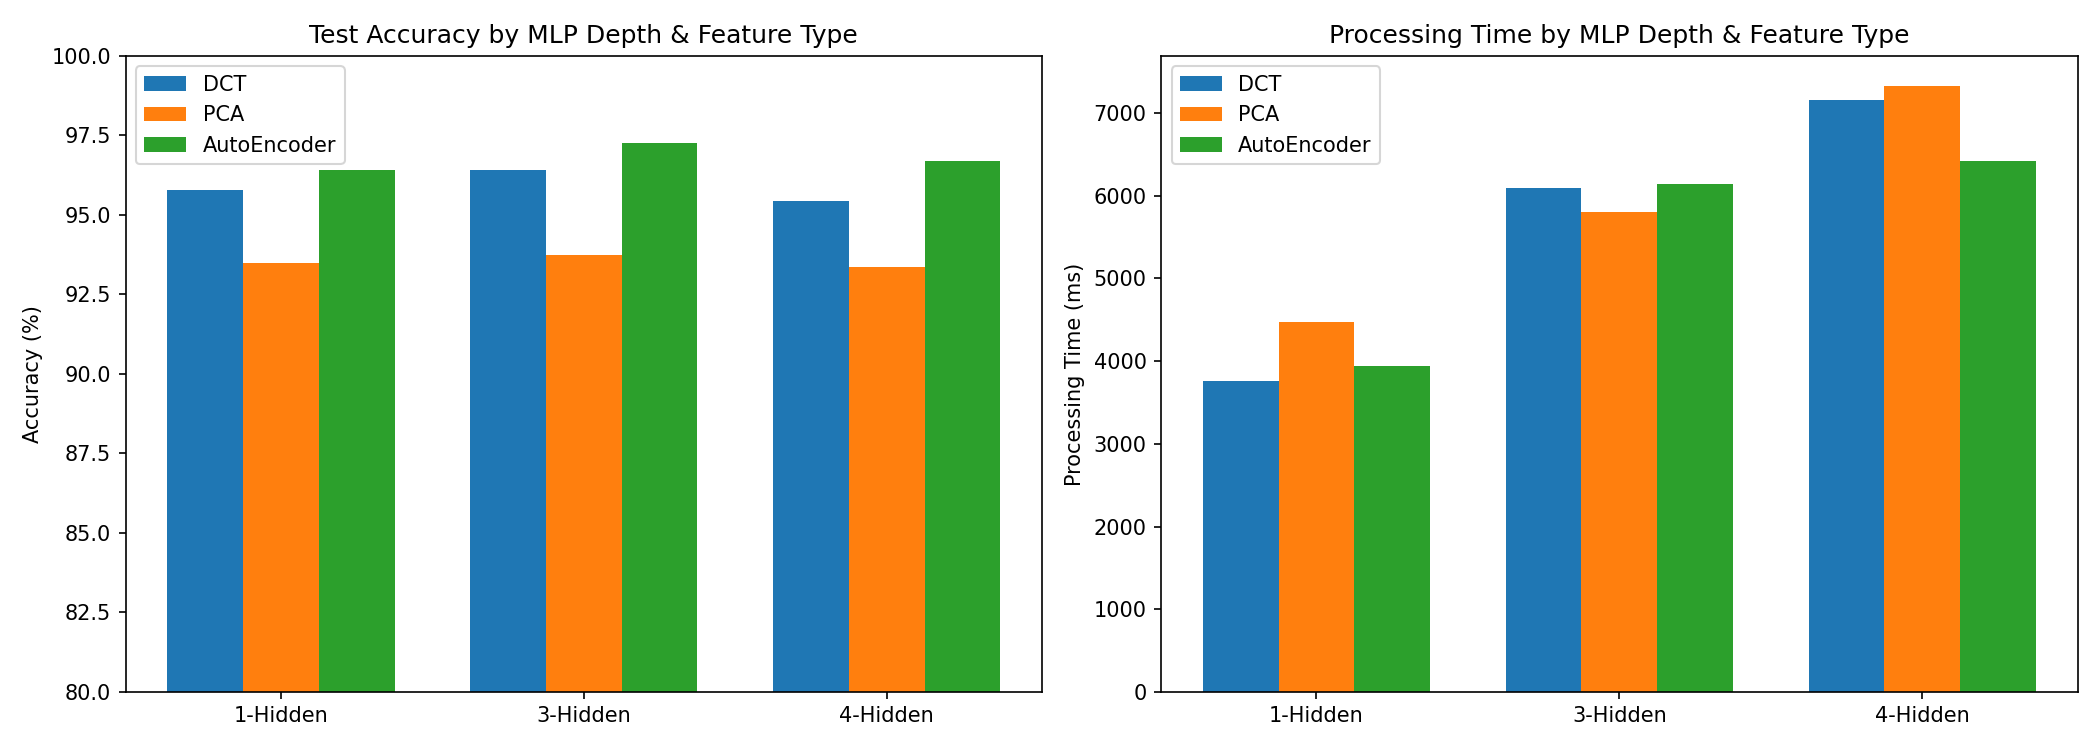
\includegraphics[width=0.95\textwidth]{mlp_results.png}
\caption{Comparison of test accuracy (left) and processing time (right) across all
         feature types and MLP depths.}
\label{fig:results}
\end{figure}

% ------------------------------------------
\subsection{Analysis and Discussion}

\subsubsection{Effect of Network Depth and Overfitting}

Increasing depth from 1 to 3 hidden layers gave a modest accuracy boost for DCT
(95.8\% $\to$ 96.4\%) and AutoEncoder (96.4\% $\to$ 97.2\%), but going to 4 hidden
layers \emph{decreased} accuracy in every feature type --- DCT dropped to 95.5\%,
PCA to 93.3\%, and AutoEncoder to 96.7\%.

This accuracy drop at 4 layers is a clear sign of \textbf{overfitting}:

\begin{itemize}
    \item \textbf{Too many parameters for the data:} the 4-layer MLP
          (256--128--64--32) has significantly more trainable weights than the
          1-layer variant.  With only 1{,}000 training samples per class,
          the extra parameters fit noise in the training set rather than
          learning generalisable patterns, leading to lower test accuracy.
    \item \textbf{Vanishing gradient effect:} deeper networks propagate
          smaller gradients to early layers, making it harder for those
          layers to learn useful features in only 10 epochs.
    \item \textbf{No regularisation:} the models use no dropout, weight
          decay, or early stopping, so deeper architectures are especially
          prone to memorising the training data.
    \item \textbf{Sweet spot at 3 layers:} the 3-layer MLP strikes the best
          balance --- enough capacity to capture non-linear patterns
          without overfitting the limited dataset.
\end{itemize}

\subsubsection{Effect of Feature Type}

The \textbf{Autoencoder features achieved the highest accuracy}
(97.2\%) despite being the smallest representation (only 64 dimensions).

\textbf{Ranking:} AutoEncoder (97.2\%) $>$ DCT (96.4\%) $>$ PCA (93.8\%)

\textbf{Why AutoEncoder outperforms:}
\begin{itemize}
    \item The autoencoder learns a \textbf{non-linear} mapping, allowing it to capture complex
          relationships between pixels that linear PCA cannot.
    \item Its 64-D features are extremely compact yet highly discriminative --- the bottleneck
          forces it to retain only the most class-relevant information.
    \item The autoencoder is trained \emph{on the same data}, so its features are tailored to
          this specific dataset.
\end{itemize}

\textbf{Why DCT outperforms PCA:}
\begin{itemize}
    \item DCT captures frequency information which is well-suited for digit recognition (global
          shape patterns).
    \item PCA with 262 components retains some noisy dimensions, which can slightly confuse the
          classifier.
\end{itemize}

\subsubsection{Processing Time}

Processing time scales with both \textbf{network depth} and \textbf{input dimensionality}:
\begin{itemize}
    \item PCA (262-D input) consistently took the longest due to the larger first weight matrix.
    \item AutoEncoder (64-D input) was the fastest despite achieving the best accuracy ---
          demonstrating that good feature engineering reduces both compute cost and error rate.
    \item Going from 1 to 4 hidden layers roughly doubles the processing time
          (e.g.\ DCT: 3758 $\to$ 7155~ms), while accuracy does not improve proportionally.
\end{itemize}

\end{document}
